\documentclass[a4paper,11pt]{book}

\usepackage{hyperref}
\usepackage{xspace}
\usepackage[T1]{fontenc}
\usepackage{palatino}
% \usepackage[dvips,dvipdf]{graphics}
\usepackage{graphics}
\usepackage{epsfig}
\usepackage{url}
\usepackage{a4wide}
\usepackage{boxedminipage}
\usepackage{calc}
\usepackage{fancybox}
\usepackage{alltt}
\usepackage{moreverb}
\usepackage{longtable}
\usepackage{array}
\usepackage{listings}
\usepackage{color}
\usepackage{rotating}
\usepackage{sectionbox}
% \usepackage{ae}
% \usepackage{aecompl}
% \usepackage[cm]{aeguill}
% \usepackage{times}
% \usepackage{bookman}
\usepackage{palatino}
%\usepackage{verbatim}

\sloppy
\newcommand{\version}{0.1}

\newcommand{\code}[1]{{\tt{#1}}}

\title{\textbf{\Huge AKANTU}\\
  \vspace{0.5cm}
  \textbf{\huge User's Guide}\\
  \vspace{1cm}
  {\small \today{} --- Version \version}
}
\date{}

\begin{document}

\maketitle

\tableofcontents

\chapter{Introduction}

\section{Data structures\label{chap:data-structure}}

\subsection{Vectors\label{sec:vectors}}

The Vector class is a template class  that can store scalar types as Real, UInt,
Int  or bool.   A Vector  instance is  defined  by its  size and  its number  of
component.  It also  has an  identifier and  some extra  internal  variables for
memory handling purpose.

\begin{itemize}
\item The size is the number of tupels stored in the Vector.
\item The number of component is the number of values stored for each tuple.
\end{itemize}

\begin{figure}[!htb]
  \centering
  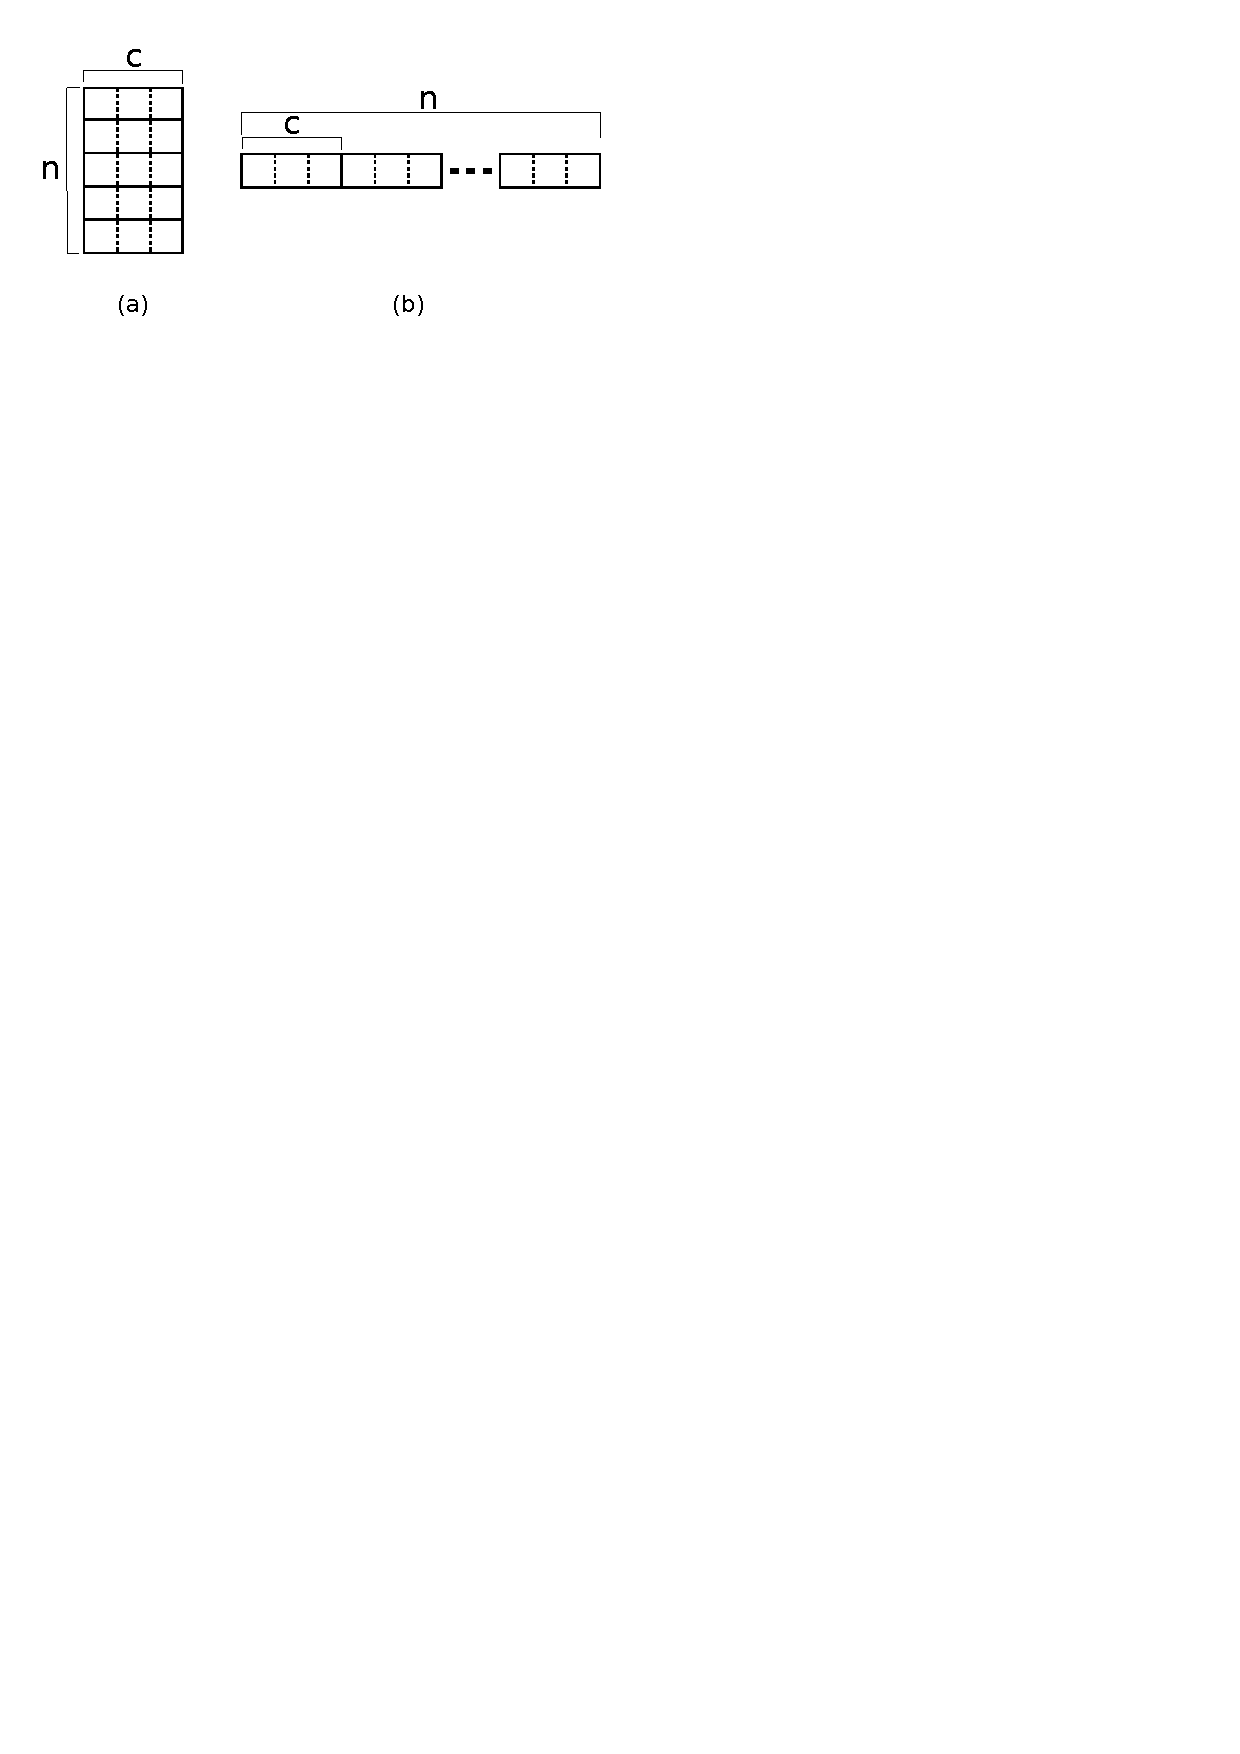
\includegraphics{figures/vectors}
  \caption{View of  a Vector of size  n and c compenents,  (a) representation of
    the vector, (b) representation of the storage of the same Vector.}
  \label{fig:vectors}
\end{figure}

All the  data are linerarized  in memory in  an array called values.  This class
member is public.  So for a Vector  of size $n$ and $c$ component, to access the
$j^{th}$  component of  th  $i^{th}$ tuple,  you have  to  get $values[i  * c  +
j]$. You  can also  access to this  value with  accessor \code{at(i, j)}  or the
constant accessor \code{get(i, j)}.

If  you want to  store a  matrix on  each tuple  you have  to linearize  it. For
exemple if you want to store a m * k matrix on each tuple you must specify c = m
* k.  To access a particular value  in a matrix of  a tuple you will  have to do
something like $values[ i * m * k + j_i * m + j_j]$.

\subsubsection{Vector storage convention within FE object\label{sec:FE-convention}}

The point of  this section is to describe the convention  of storage for vectors
intented  to be  passed to  {\bf  FE} object  methods.  Indeed  a convention  of
necessary  since gradient  operators or  integration loops  will use  vectors as
input and ouput.   Such vectors will be ordered with  a specific convention that
we intend to describe now.

For  vector objects,  the  size of  the vector  is  always the  number of  nodes
associated.  The number  of components  is related  to the  order of  the tensor
considered. For a scalar  field it is 1, for a vectorial  field, the size of the
vector is the number of components. For a $m\times n$ matrix field the number of
components is $m\times n$.

One common operation  is the manipulation of continuum  fields at the quadrature
point  positions.   Here  the  size   of  the  vector  is   $mn\_element  \times
nb\_quad\_points$  and  the  number  of  components is  related  to  the  stored
object.  For instance the  method \verb$interpolateOnQuadraturePoints()$  take a
nodal field  stored in a  vector($n\_nodes$,$dim$) and return  a vector($n\_elem
\times n\_quads$,$dim$).

Basic gradient operations, like method \verb$gradientOnQuadraturePoints()$, will
take  as input a  vector($n\_nodes$,$dim$) and  return a  vector($n\_elem \times
n\_quads$,$dim \times spatial\_dimension$) where spatial dimension is the number
of dimension in which the domain is embedded.

In  the  same  way   the  integration  routines  expect  vector($n\_elem  \times
n\_quads$,$dim$)  and  will  return vector($n\_elem$,$dim$).   For  non-Gaussian
integrations, the input  by be direction a nodal field.   (At present time, only
gaussian integrators are implemented within akantu).

Last but  not the least  is the vectorial  assembly process for which  accept as
input vector($n\_elem \times n\_quads \times n\_nodes\_per\_element$,$dim$)
and will return a vector($n\_nodes$,$dim$) nodal object.\\

{\bf The general convention is that  the number of component shall always be the
  size of  the object manipulated  at the lowest  level.  The object could  be a
  per-element, of  per quadrature point  or even per  node basis this  will also
  apply    as   shown    below.   The    figures    \ref{fig:vector-chain}   and
  \ref{fig:interpolate-storage} shows the  pattern of the vectors is  the case a
  interpolation on quadrature points.}

\begin{figure}
  \begin{equation}
    \left(
      \begin{array}{c}
	N_1 \\
	\vdots \\
	N_I
	\left\{
	  \begin{array}{c}
	    a_1 \\
	    \vdots \\
	    a_{dim} \\
	  \end{array}
	\right. \\
	\vdots \\
	N_{nb\_nodes}
      \end{array}
    \right)
    \begin{array}{c}
      \Longrightarrow \\
      interpolate\\
      On\\
      Quadrature\\
      Points\\
    \end{array}
    \left(
      \begin{array}{c}
	E_1 \\
	\vdots \\
	E_e
	\left\{
	  \begin{array}{c}
	    q_1 \\
	    \vdots \\
	    \left.
	      \begin{array}{c}
		a_1 \\
		\vdots \\
		a_{dim}
	      \end{array}
	    \right\} q_i \\
	    \vdots \\
	    q_p \\
	  \end{array}
	\right.  \\
	\vdots \\
	E_{nb\_elements}
      \end{array}
    \right)
  \end{equation}
  \caption{\label{fig:vector-chain}Pattern   of   vectors   manipulated   during
    interpolation on  quadrature points.  Symbols  N (resp. E, q)  denotes nodes
    (resp. elements, quadrature points).}
\end{figure}

\begin{figure}[!htb]
  \centering
  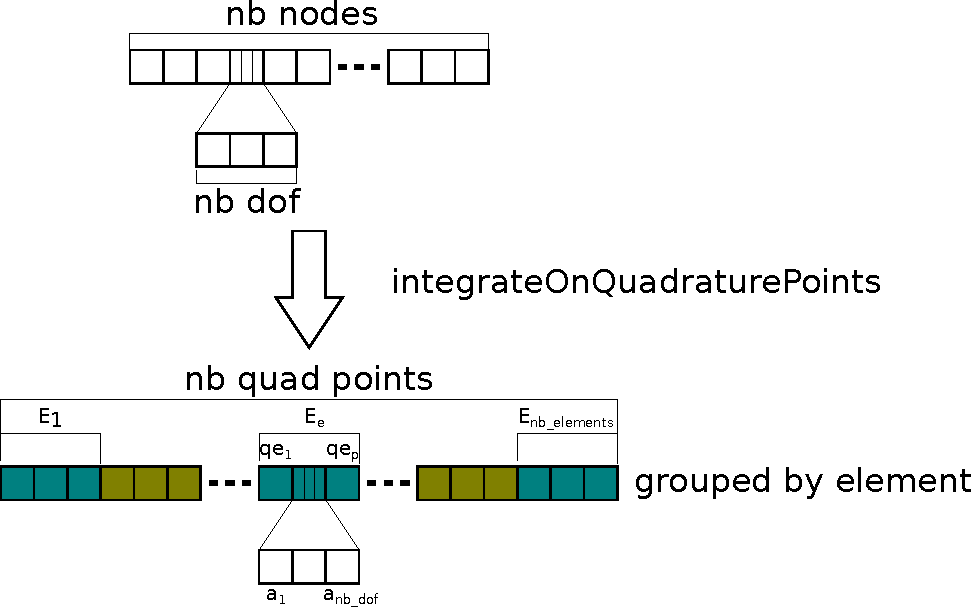
\includegraphics{figures/interpolate}
  \caption{Input and output  vector of interpolateOnQuadraturePoints. The output
    Vector has nb\_quadrature\_points tuples,  the quadrature points are grouped
    by elements (p is the number of quadrature points per element).}
  \label{fig:interpolate-storage}
\end{figure}


\chapter{How to use Akantu}

\section{Solid Mechanics model}

The  solid  mechanics  model  is   a  specifique  implementation  of  the  model
interface. The model is instanciated for a given mesh. It will create is own FEM
object   to   do  the   interpolation,   gradient,   integration  and   assemble
operations. This model contain some Vectors that we will describe now.

\begin{itemize}
\item[Displacement] contain the  displacements of the free degrees  of freedom or
  the imposed displacements for the blocked degrees of freedom.
\item[Velocity] contain the velocities of  the degree of freedoms, acts like the
  displacement vector
\item[Acceleration] contain  the accelerations of  the degree of  freedoms, acts
  like the displacement vector
\item[Force] contain the external forces applied on the different nodes.
\end{itemize}

\subsection{Resolution methods}
\subsubsection{Implicit static}

\subsubsection{Implicit dynamic}

\subsubsection{Explicit}

\subsection{Constitutive laws}
\subsection{}
\subsection{Contact}

\subsection{Cohesive laws}


\section{Structural Mechanics model}

\section{Heat Transfer model}

% \subsection{Contact Neighbor Structure}

% The contact neighbor  structure is an interface which is  ment to be heritated
% from in order  to implement different type of  contact neighbor structures. It
% has the following protected attributes:
% \begin{itemize}
%   \item id
%   \item contact search
%   \item master surface
%   \item neighbor list
%   \item type
% \end{itemize}
% The \emph{id} and the \emph{type}  are characteristics of the contact neighcor
% structure object which  define its id and its  type. The \emph{contact search}
% attribute  is  the associated  contact  search  object  to the  given  contact
% neighbor structure  object. The \emph{master  surface} attribute is the  id of
% the  associated master  surface for  which the  neighbor structure  has  to be
% built. Finally, the neighbor list  is the constructed neighbor structure which
% defines the  impactor nodes  that are  in the neighborhood  of either  a given
% master  node or  a given  master  surface element,  depending on  the type  of
% contact neighbor structure.

% The contact neighbor structure provides the accessor \emph{getNeighborList} to
% the constructed  neighbor list and forces  the heritated classes  to provide a
% public \emph{initNeighborStructure}  function, which initializes  the neighbor
% structure,  as well  as a  public  \emph{update} function,  which updates  the
% neighbor structure.

% \subsubsection{Regular Grid Neighbor Structure}

% The regular  grid neighbor structure builds  a regular grid  around the master
% surface and  uses it in  order to construct  the neighbor list.  This neighbor
% structure can construct both types of neighbor list, the


% \subsection{Implementation of a new solid mechanics problem}

% Let us imagine you want to implement a new material called
% "toto" in akantu. The have to complete the following steps (in
% any order) :
% \begin{enumerate}
% \item
% Declare a new material in the file
%      \textit{Akantu/model/solid\_mechanics/solid\_mechanics\_model\_material.cc}.
% You have to had this line after the list of possible cases
% \begin{verbatim}else if(mat\_type == "toto") material =
%      parser.readMaterialObject<MaterialToto>(*this,mat_id);
% \end{verbatim}


% \item
% Include the new material in \textit{Akantu/model/solid\_mechanics/material.hh} \\
% add the line :
% \begin{verbatim}
% #include "materials/material\_toto.hh"
% \end{verbatim}

% \item
% For compilation include the new file to compile in
%      \textit{Akantu/CMakelist.txt} by adding
% \begin{verbatim}
% model/solid_mechanics/materials/material_toto.cc
% \end{verbatim}
% \item
% In \textit{Akantu/model/solid\_mechanics/materials}, create (or copy from
%      an allready existing material) the three following files :\\
% - material\_toto.cc\\
% - material\_toto.hh\\
% - material\_toto\_inline\_impl.cc

% \item
% Modify the files !

% \end{enumerate}

\end{document}
